\documentclass[12pt]{article}
\usepackage[utf8]{inputenc}
\usepackage{graphicx}
\usepackage{hyperref}
\usepackage{listings}
\usepackage{xcolor}
\usepackage{geometry}
\usepackage{enumitem}
\usepackage{amsmath}
\usepackage{amssymb}
\usepackage{longtable}
\usepackage{booktabs}
\usepackage{titlesec}
\usepackage{tikz}
\usetikzlibrary{shapes.geometric, arrows.meta, positioning, fit, backgrounds, calc}

\geometry{a4paper, margin=1in}
\setlength{\parindent}{0pt}
\setlength{\parskip}{0.5em}

\hypersetup{
    colorlinks=true,
    linkcolor=blue!70!black,
    urlcolor=blue!60!black,
}

\title{Technical Documentation\\[0.3em]
\large orthodox.net Flask Backend}
\author{Generated Documentation}
\date{\today}

\lstset{
    basicstyle=\ttfamily\small,
    breaklines=true,
    frame=tb,
    framesep=4pt,
    language=Python,
    numbers=left,
    numberstyle=\tiny,
    keywordstyle=\color{blue},
    commentstyle=\color{green!60!black},
    stringstyle=\color{red},
    showstringspaces=false
}

\lstdefinelanguage{SQL}{
    keywords={CREATE, TABLE, IF, NOT, EXISTS, PRIMARY, KEY, UNIQUE, DEFAULT, NOW, INDEX, ON, REFERENCES, DELETE, CASCADE, USING, SERIAL, TEXT, INTEGER, TIMESTAMP, WITH, TIME, ZONE, JSONB, VARCHAR, DATE, INTERVAL, RETURNS, AS, BEGIN, END, LANGUAGE, OR, REPLACE, FUNCTION, GIN, DESC},
    keywordstyle=\color{blue}\bfseries,
    commentstyle=\color{green!60!black},
    stringstyle=\color{red},
    morecomment=[l]{--},
    sensitive=false,
}

\begin{document}
\sloppy

\maketitle

\begin{abstract}
This document is a comprehensive technical reference for the orthodox.net Flask Backend --- a Python/Flask REST API that aggregates content from Ghost CMS, YouTube, and Google Calendar into a unified JSON interface for the St.\ Nicholas Orthodox Church website. The application is deployed on Render.com with staging and production environments, and uses Supabase (PostgreSQL) as a caching layer to reduce external API quota usage. This reference is intended for senior/full-stack developers and DevOps engineers who need to understand, maintain, deploy, or extend the application. It covers system architecture with dependency diagrams, complete API endpoint documentation with request/response examples, database schemas for both cache tables, caching strategy with TTL configuration and error fallback behavior, core module internals, Render.com deployment configuration with service IDs and URLs, environment variable and credential management, error handling patterns, logging infrastructure, security considerations, known technical debt, a maintenance checklist for project continuity, and the full project history organized by development milestone.
\end{abstract}

\tableofcontents
\newpage

%% ============================================================
\section{Executive Summary}
%% ============================================================
{\setlength{\parskip}{0pt}\setlength{\parfillskip}{0pt plus 1fil}%
\titlespacing*{\paragraph}{0pt}{0.6ex plus 0.2ex minus 0.1ex}{0.5em}%

\textbf{orthodox.net} is the website of St.\ Nicholas Orthodox Church in McKinney, Texas. The orthodox.net Flask Backend is a Python/Flask REST API that serves as the data layer for the site, aggregating content from Ghost CMS, YouTube, and Google Calendar into a unified JSON interface consumed by the frontend. The project began in September 2023 and has evolved through seven development phases, from an initial Heroku deployment to the current Render.com infrastructure with Supabase caching.

\paragraph{Architecture.} The backend is a single Flask application (\texttt{app.py}) deployed on Render.com with Gunicorn as the WSGI server. External integrations are organized into separate modules: \texttt{fetch\_ghost.py} for articles, \texttt{fetch\_youtube.py} for videos, and \texttt{fetch\_calendar.py} for church events. Each cached integration has a dedicated cache module (\texttt{calendar\_cache.py}, \texttt{video\_cache.py}) backed by Supabase (PostgreSQL). Calendar events are cached for 24 hours and YouTube videos for 6 hours, significantly reducing external API quota consumption. The API is public with no authentication; CORS is open to all origins. Interactive Swagger documentation is auto-generated via Flasgger and available at the \texttt{/docs} endpoint.

\paragraph{API Surface.} The backend exposes endpoints across three content domains: articles from Ghost CMS (\texttt{/onet\_articles}, \texttt{/onet\_article}, \texttt{/article\_by\_slug}, \texttt{/parish\_life}, \texttt{/motd}, and others), videos from YouTube (\texttt{/latest\_videos} with caching, plus playlist endpoints for homilies, children's sermons, and catechism), and calendar events from Google Calendar (\texttt{/schedule} with caching). Admin endpoints (\texttt{POST /cache\_videos}, \texttt{/view\_video\_cache}) allow manual cache management. A legacy article scraper fetches historical content from the original \texttt{orthodox.net} site by extracting HTML between comment markers.

\paragraph{Deployment.} The application runs on two Render.com Web Services (Starter plan, Virginia region): \texttt{production-orthodox-net-flask} (deployed from the \texttt{main} branch) and \texttt{staging-orthodox-net-flask} (deployed from \texttt{staging}). Both auto-deploy on push to their respective branches. Environment variables for Supabase and Google Calendar are configured per-service in the Render dashboard. Ghost CMS and YouTube credentials are currently hardcoded in source files rather than read from environment variables --- migrating these is a known technical debt item.

\paragraph{Technology Stack.} Python 3.12.3, Flask 2.1.2, Werkzeug 2.0.3, Gunicorn; Supabase (PostgreSQL) for caching; \texttt{requests} for HTTP calls to Ghost CMS and YouTube; \texttt{google-api-python-client} for Calendar; \texttt{python-dotenv} for environment management; \texttt{beautifulsoup4} for HTML parsing; \texttt{pytz} for US/Central timezone handling. Testing uses pytest with pytest-mock and pytest-cov.

\paragraph{This Document.} This technical reference covers system architecture, all API endpoints with request/response examples, database schemas, caching strategies, module internals, deployment configuration, error handling, logging, security considerations, and known technical debt. Section~\ref{sec:checklist} provides a maintenance checklist; Appendix~\ref{sec:history} provides the project history by milestone; Appendix~\ref{sec:revisions} records this document's revision history.

\vspace{1em}
\begin{center}
\footnotesize
Repository: \url{https://github.com/GZancewicz/onet-flask-backend}\\
Production: \url{https://production-orthodox-net-flask.onrender.com}\\
Staging: \url{https://staging-orthodox-net-flask.onrender.com}
\end{center}
}% end parskip group

\clearpage
%% ============================================================
\section{Introduction}
%% ============================================================

The orthodox.net Flask Backend is a REST API that aggregates content from multiple external services and presents a unified interface to frontend clients. It powers the orthodox.net platform for St.\ Nicholas Orthodox Church.

\subsection{Source Repository}
The source code is hosted on GitHub at:

\begin{center}
\url{https://github.com/GZancewicz/onet-flask-backend}
\end{center}

\noindent The \texttt{main} branch is deployed to production and \texttt{staging} to the staging environment (both on Render.com). All pull requests should target \texttt{main} unless specifically intended for staging testing. For a narrative overview of the project's development history, see Appendix~\ref{sec:history}.

\subsection{What This Application Does}
\begin{enumerate}
    \item \textbf{Article management} --- Proxies articles from a Ghost CMS instance, with tag-based filtering, slug lookups, and heading reformatting for frontend consumption.
    \item \textbf{Video aggregation} --- Fetches and caches YouTube videos from the church's channel and curated playlists (homilies, children's sermons, catechism).
    \item \textbf{Calendar integration} --- Retrieves upcoming church events from Google Calendar, formats them with human-readable dates/times, and caches results.
    \item \textbf{Legacy content} --- Scrapes historical articles from the legacy \texttt{orthodox.net} website.
\end{enumerate}

\subsection{Architecture Goals}
\begin{itemize}
    \item Single deployment artifact (one Flask app, one Gunicorn process)
    \item Minimize external API calls through Supabase caching (YouTube and Google Calendar have strict quotas)
    \item CORS-open so any frontend can consume the API
    \item Self-documenting via Swagger UI at \texttt{/docs}
    \item Comprehensive logging for debugging production issues
\end{itemize}

%% ============================================================
\section{System Architecture}
%% ============================================================

\subsection{High-Level Overview}

\begin{figure}[ht]
\centering
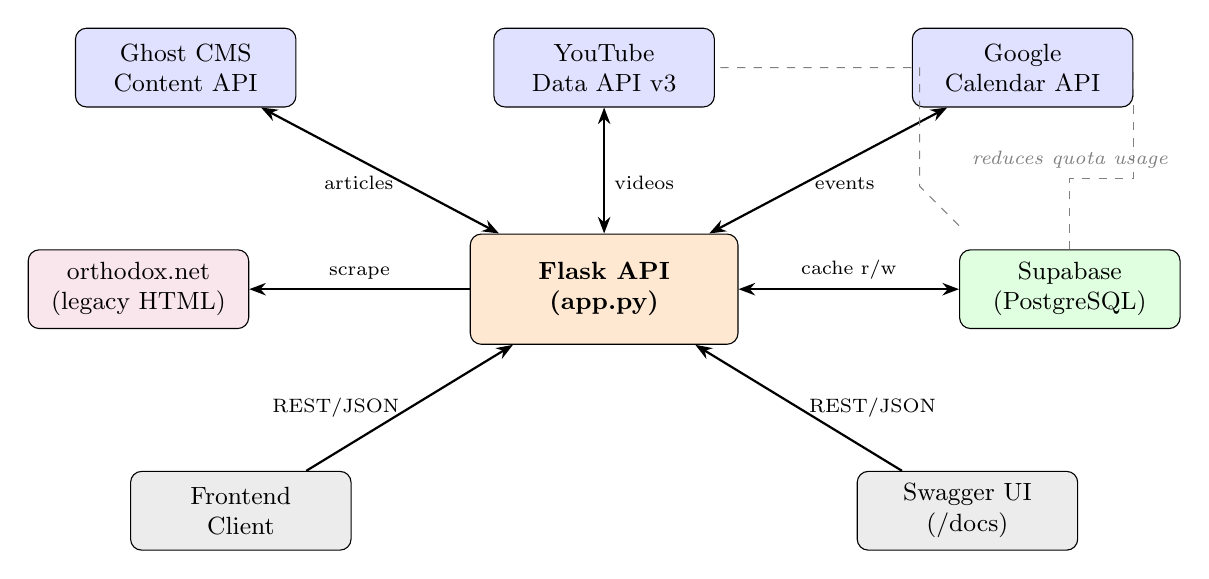
\begin{tikzpicture}[
    node distance=1.8cm and 2.5cm,
    box/.style={rectangle, draw, rounded corners, minimum width=2.8cm, minimum height=1cm, align=center, font=\small},
    extapi/.style={box, fill=blue!12},
    cache/.style={box, fill=green!12},
    app/.style={box, fill=orange!18, minimum width=3.4cm, minimum height=1.4cm, font=\small\bfseries},
    client/.style={box, fill=gray!15},
    legacy/.style={box, fill=purple!10},
    arr/.style={-{Stealth[length=6pt]}, thick},
    dualarr/.style={{Stealth[length=6pt]}-{Stealth[length=6pt]}, thick},
]
    % Central app
    \node[app] (flask) {Flask API\\(app.py)};

    % External APIs (top row)
    \node[extapi, above left=1.6cm and 2.2cm of flask]  (ghost)    {Ghost CMS\\Content API};
    \node[extapi, above=1.6cm of flask]                  (youtube)  {YouTube\\Data API v3};
    \node[extapi, above right=1.6cm and 2.2cm of flask]  (calendar) {Google\\Calendar API};

    % Legacy (far left)
    \node[legacy, left=2.8cm of flask] (legacysite) {orthodox.net\\(legacy HTML)};

    % Cache (right)
    \node[cache, right=2.8cm of flask] (supabase) {Supabase\\(PostgreSQL)};

    % Clients (bottom)
    \node[client, below left=1.6cm and 1.5cm of flask]  (frontend) {Frontend\\Client};
    \node[client, below right=1.6cm and 1.5cm of flask] (swagger)  {Swagger UI\\(/docs)};

    % Arrows: app to external APIs
    \draw[dualarr] (flask) -- node[left, font=\scriptsize, pos=0.4] {articles} (ghost);
    \draw[dualarr] (flask) -- node[right, font=\scriptsize, pos=0.4] {videos} (youtube);
    \draw[dualarr] (flask) -- node[right, font=\scriptsize, pos=0.4] {events} (calendar);

    % Arrows: app to legacy
    \draw[arr] (flask) -- node[above, font=\scriptsize] {scrape} (legacysite);

    % Arrows: app to cache
    \draw[dualarr] (flask) -- node[above, font=\scriptsize] {cache r/w} (supabase);

    % Arrows: clients to app
    \draw[arr] (frontend) -- node[left, font=\scriptsize] {REST/JSON} (flask);
    \draw[arr] (swagger)  -- node[right, font=\scriptsize] {REST/JSON} (flask);

    % Dashed lines: cache reduces calls
    \draw[dashed, gray] (supabase.north) -- ++(0, 0.9) node[above, font=\scriptsize\itshape, text=gray] {reduces quota usage} -| (calendar.east);
    \draw[dashed, gray] (supabase.north west) ++(0, 0.3) -- ++(-0.5, 0.5) |- ($(youtube.east)+(0.3,0)$) -- (youtube.east);
\end{tikzpicture}
\caption{System architecture. The Flask API is the central hub. Supabase caches YouTube and Calendar data to stay within API quotas. Ghost CMS and legacy site are called directly on every request (no caching).}
\label{fig:architecture}
\end{figure}

\subsection{Core Technology Stack}

\begin{longtable}{lll}
\toprule
\textbf{Component} & \textbf{Version} & \textbf{Purpose} \\
\midrule
\endhead
Flask & 2.1.2 & Web framework \\
Werkzeug & 2.0.3 & WSGI utilities (pinned for Flask 2.1 compat) \\
Flasgger & 0.9.7.1 & Swagger UI auto-generation \\
flask\_cors & 4.0.0 & CORS middleware \\
Gunicorn & (latest) & Production WSGI server \\
requests & 2.28.2 & HTTP client for Ghost, YouTube, legacy site \\
google-api-python-client & 2.91.0 & Google Calendar API client \\
supabase & 2.18.0 & Supabase Python client \\
SQLAlchemy & 2.0.23 & Database ORM (used in \texttt{db/} setup scripts) \\
psycopg2-binary & 2.9.10 & PostgreSQL adapter \\
pytz & 2023.3 & Timezone conversions (US/Central) \\
python-dotenv & 1.0.1 & \texttt{.env} file loading \\
beautifulsoup4 & 4.12.3 & HTML parsing \\
pytest & 7.4.3 & Test framework \\
pytest-mock & 3.11.1 & Mock fixtures for tests \\
pytest-cov & 4.1.0 & Coverage reporting \\
Python & 3.12.3 & Runtime (specified in \texttt{runtime.txt}) \\
\bottomrule
\end{longtable}

\subsection{Module Dependency Graph}

\begin{figure}[p]
\centering
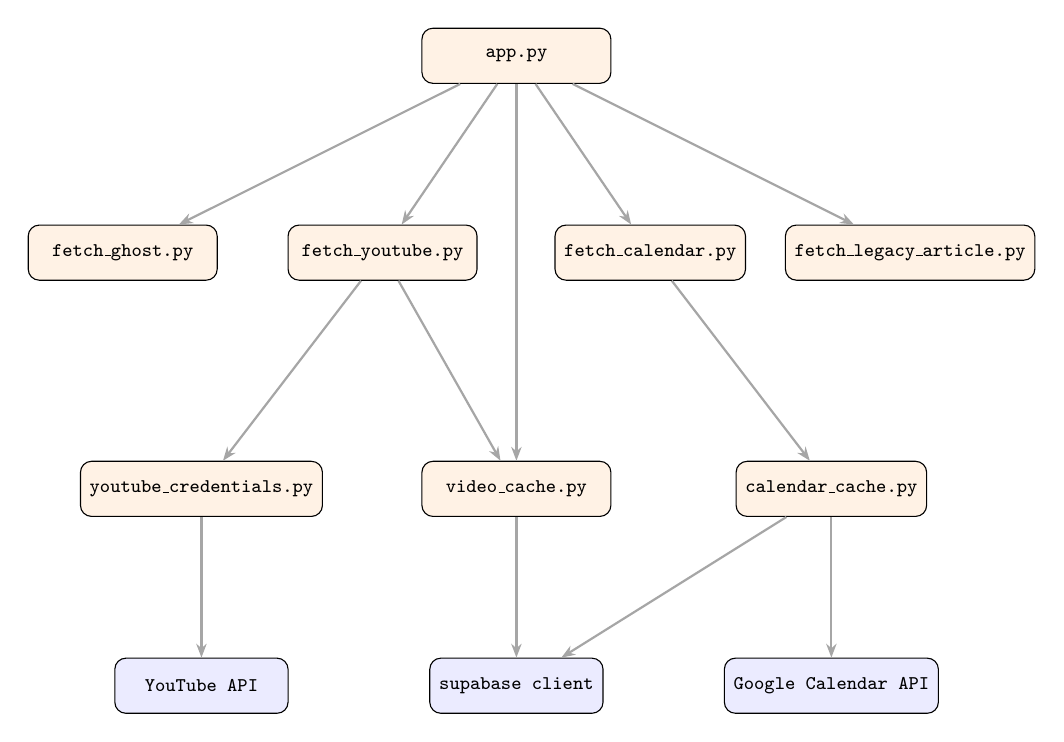
\begin{tikzpicture}[
    mod/.style={rectangle, draw, rounded corners, fill=orange!10, minimum width=2.4cm, minimum height=0.7cm, align=center, font=\scriptsize\ttfamily},
    ext/.style={rectangle, draw, rounded corners, fill=blue!8, minimum width=2.2cm, minimum height=0.7cm, align=center, font=\scriptsize\ttfamily},
    arr/.style={-{Stealth[length=5pt]}, thick, gray!70},
]
    % Row 1: app.py (centered at 0,0)
    \node[mod] (app) at (0, 0) {app.py};

    % Row 2: four fetch modules at explicit x positions
    \node[mod] (fghost) at (-5, -2.5) {fetch\_ghost.py};
    \node[mod] (fyt)    at (-1.7, -2.5) {fetch\_youtube.py};
    \node[mod] (fcal)   at (1.7, -2.5) {fetch\_calendar.py};
    \node[mod] (fleg)   at (5, -2.5) {fetch\_legacy\_article.py};

    % Row 3: cache/credential modules with wide spacing
    \node[mod] (ytcred) at (-4, -5.5) {youtube\_credentials.py};
    \node[mod] (vcache) at (0, -5.5) {video\_cache.py};
    \node[mod] (ccache) at (4, -5.5) {calendar\_cache.py};

    % Row 4: external services with wide spacing
    \node[ext] (ytapi) at (-4, -8) {YouTube API};
    \node[ext] (supa)  at (0, -8) {supabase client};
    \node[ext] (gcal)  at (4, -8) {Google Calendar API};

    % Arrows from app to fetch modules
    \draw[arr] (app) -- (fghost);
    \draw[arr] (app) -- (fyt);
    \draw[arr] (app) -- (fcal);
    \draw[arr] (app) -- (fleg);
    \draw[arr] (app.south) -- ++(0,-0.8) -| (vcache);

    % Arrows from fetch modules to their dependencies
    \draw[arr] (fyt) -- (ytcred);
    \draw[arr] (fyt) -- (vcache);
    \draw[arr] (fcal) -- (ccache);

    % Arrows to external services
    \draw[arr] (ytcred) -- (ytapi);
    \draw[arr] (vcache) -- (supa);
    \draw[arr] (ccache) -- (supa);
    \draw[arr] (ccache) -- (gcal);
\end{tikzpicture}
\caption{Module dependency graph. Each fetch module has its own cache module backed by Supabase.}
\label{fig:modules}
\end{figure}

\clearpage
\subsection{Project Structure}
\begin{lstlisting}[language={}, basicstyle=\ttfamily\footnotesize, frame=none, numbers=none]
onet-flask-backend/
|-- app.py                     # Main Flask app, all REST endpoints
|-- fetch_ghost.py             # Ghost CMS Content API client
|-- fetch_youtube.py           # YouTube Data API v3 client + caching
|-- youtube_credentials.py     # YouTube API key (hardcoded)
|-- fetch_calendar.py          # Google Calendar API client + caching
|-- calendar_cache.py          # Supabase ops for calendar_events table
|-- video_cache.py             # Supabase ops for youtube_videos table
|-- fetch_legacy_article.py    # Scrapes orthodox.net legacy HTML
|-- conftest.py                # Pytest configuration
|-- db/
|   |-- src/
|   |   |-- setup_db.py              # DB initialization via SQLAlchemy
|   |   +-- setup_youtube_tables.py  # YouTube table creation
|   +-- test/                        # DB setup tests
|-- modules/
|   +-- youtube/
|       |-- src/fetch_youtube.py     # Alternate YouTube module
|       +-- test/                    # Unit + live integration tests
|-- test/                      # Main test suite
|-- legacy_test/               # Legacy tests (Ghost, YouTube)
|-- data/bulletin/             # Bulletin PDF extraction utilities
|-- util/onet-v2-utils/        # Misc utility scripts
|-- db_schema.sql              # Calendar + YouTube table schemas
|-- video_cache_schema.sql     # Video cache table (simplified schema)
|-- requirements.txt           # Python dependencies (used by Render)
|-- runtime.txt                # Python version for Render (3.12.3)
|-- Procfile                   # Gunicorn start command (legacy Heroku
|                              #   format, still used by Render)
|-- .env.sample                # Environment variable template
+-- doc/
    +-- latex/onet_backend/    # This document (LaTeX + PDF + compile script)
\end{lstlisting}

\textbf{Note on Procfile:} The \texttt{Procfile} was originally created for Heroku. Render.com also reads this file format, so it remains functional. It contains a single line: \texttt{web: gunicorn app:app}. If migrating to a different hosting platform, this file may need to be replaced with the platform's equivalent (e.g., a Dockerfile, \texttt{render.yaml}, etc.).

%% ============================================================
\section{Database Layer}
%% ============================================================

The application uses Supabase (hosted PostgreSQL) exclusively as a caching layer. There is no user data, authentication, or transactional data stored.

\subsection{Database Schema}

Two SQL files define the schema. Both should be run in the Supabase SQL editor during initial setup.

\subsubsection{Calendar Events Table (\texttt{db\_schema.sql})}

\begin{lstlisting}[language=SQL, basicstyle=\ttfamily\footnotesize]
CREATE TABLE IF NOT EXISTS calendar_events (
    id            SERIAL PRIMARY KEY,
    event_id      VARCHAR(255) UNIQUE NOT NULL,
    summary       TEXT,
    start_time    TIMESTAMP WITH TIME ZONE,
    end_time      TIMESTAMP WITH TIME ZONE,
    location      TEXT,
    description   TEXT,
    raw_data      JSONB,
    date_key      DATE NOT NULL,
    cached_at     TIMESTAMP WITH TIME ZONE DEFAULT NOW(),
    UNIQUE(event_id, date_key)
);

CREATE INDEX idx_calendar_events_date
    ON calendar_events(date_key);
CREATE INDEX idx_calendar_events_cached
    ON calendar_events(cached_at);
\end{lstlisting}

\textbf{Key design decisions:}
\begin{itemize}
    \item \texttt{event\_id} is the Google Calendar event ID; upserts use \texttt{ON CONFLICT event\_id}.
    \item \texttt{date\_key} enables fast date-range queries without parsing \texttt{start\_time}.
    \item \texttt{raw\_data} stores the complete Google Calendar API response as JSONB, so the application can re-extract any field without a schema migration.
    \item \texttt{cached\_at} is compared against \texttt{CACHE\_TTL\_HOURS} (default 24) to determine staleness.
\end{itemize}

\subsubsection{YouTube Videos Table (\texttt{video\_cache\_schema.sql})}

\begin{lstlisting}[language=SQL, basicstyle=\ttfamily\footnotesize]
CREATE TABLE IF NOT EXISTS youtube_videos (
    video_id    TEXT PRIMARY KEY,
    title       TEXT,
    description TEXT,
    thumbnail_url TEXT,
    published_at  TIMESTAMP,
    channel_id    TEXT,
    playlist_id   TEXT,
    video_type    TEXT,   -- 'latest','homilies','childrens','catechism'
    raw_data      JSONB,
    cached_at     TIMESTAMP DEFAULT NOW()
);

CREATE INDEX IF NOT EXISTS idx_youtube_videos_type
    ON youtube_videos(video_type);
CREATE INDEX IF NOT EXISTS idx_youtube_videos_cached_at
    ON youtube_videos(cached_at);
CREATE INDEX IF NOT EXISTS idx_youtube_videos_playlist
    ON youtube_videos(playlist_id);
\end{lstlisting}

A PostgreSQL function for periodic cleanup is also defined:
\begin{lstlisting}[language=SQL, basicstyle=\ttfamily\footnotesize]
CREATE OR REPLACE FUNCTION clean_old_video_cache()
RETURNS void AS $$
BEGIN
    DELETE FROM youtube_videos
    WHERE cached_at < NOW() - INTERVAL '7 days';
END;
$$ LANGUAGE plpgsql;
\end{lstlisting}

\subsubsection{Additional Tables in \texttt{db\_schema.sql} (Future Use)}

The \texttt{db\_schema.sql} file also defines two additional tables that are provisioned but \textbf{not yet used} by the application code:

\begin{itemize}
    \item \texttt{youtube\_videos} --- A more detailed YouTube table with \texttt{playlist\_ids TEXT[]}, \texttt{tags TEXT[]}, \texttt{metadata JSONB}, and \texttt{updated\_at}. This overlaps with \texttt{video\_cache\_schema.sql}; the simpler schema is what \texttt{video\_cache.py} actually uses.
    \item \texttt{youtube\_transcriptions} --- Planned table for storing video transcriptions with full-text search (\texttt{GIN} index on \texttt{to\_tsvector}). Foreign-keyed to the YouTube videos table.
\end{itemize}

%% ============================================================
\section{Caching Layer}
%% ============================================================

\subsection{Cache Strategy}

\begin{figure}[p]
\centering
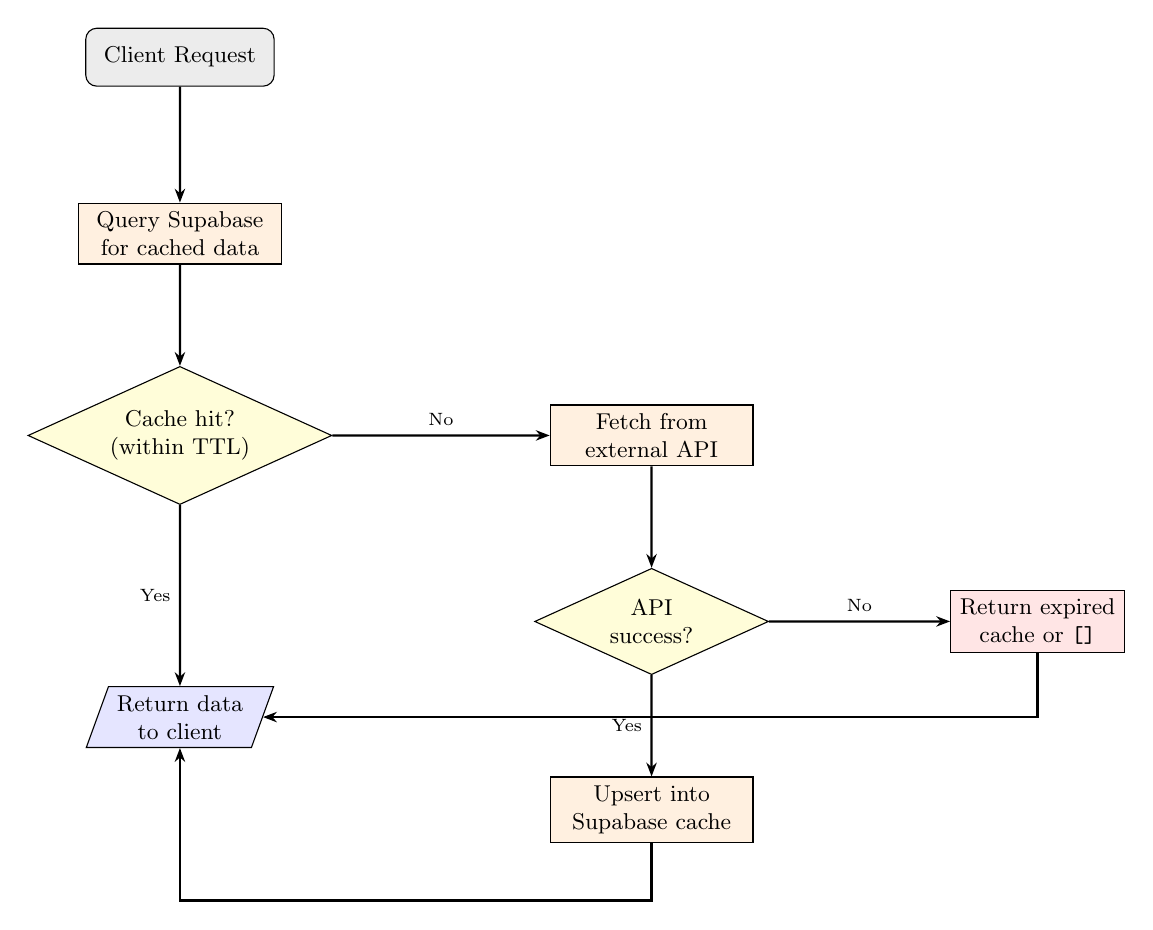
\begin{tikzpicture}[scale=0.92, every node/.style={transform shape},
    node distance=1.6cm,
    startstop/.style={rectangle, rounded corners, draw, fill=gray!15, minimum width=2.6cm, minimum height=0.8cm, align=center, font=\small},
    process/.style={rectangle, draw, fill=orange!12, minimum width=2.8cm, minimum height=0.8cm, align=center, font=\small},
    decision/.style={diamond, draw, fill=yellow!15, minimum width=2cm, minimum height=1.4cm, align=center, font=\small, aspect=2.2},
    io/.style={trapezium, trapezium left angle=70, trapezium right angle=110, draw, fill=blue!10, minimum width=2.4cm, minimum height=0.8cm, align=center, font=\small},
    fail/.style={rectangle, draw, fill=red!10, minimum width=2.4cm, minimum height=0.8cm, align=center, font=\small},
    arr/.style={-{Stealth[length=5pt]}, thick},
]
    \node[startstop] (start) {Client Request};
    \node[process, below=of start] (check) {Query Supabase\\for cached data};
    \node[decision, below=1.4cm of check] (cached) {Cache hit?\\(within TTL)};
    \node[io, below=2.5cm of cached] (respond) {Return data\\to client};
    \node[process, right=3cm of cached] (fetch) {Fetch from\\external API};
    \node[decision, below=1.4cm of fetch] (ok) {API\\success?};
    \node[process, below=1.4cm of ok] (store) {Upsert into\\Supabase cache};
    \node[fail, right=2.5cm of ok] (fallback) {Return expired\\cache or \texttt{[]}};

    \draw[arr] (start) -- (check);
    \draw[arr] (check) -- (cached);
    \draw[arr] (cached) -- node[left, font=\scriptsize] {Yes} (respond);
    \draw[arr] (cached) -- node[above, font=\scriptsize] {No} (fetch);
    \draw[arr] (fetch) -- (ok);
    \draw[arr] (ok) -- node[left, font=\scriptsize] {Yes} (store);
    \draw[arr] (store.south) -- ++(0,-0.8) -| (respond);
    \draw[arr] (ok) -- node[above, font=\scriptsize] {No} (fallback);
    \draw[arr] (fallback.south) |- (respond);
\end{tikzpicture}
\caption{Cache lookup flow with error fallback. On API failure, the calendar module returns expired cache data; the video module returns an empty list.}

\label{fig:cacheflow}
\end{figure}

\subsection{Calendar Events Cache (\texttt{calendar\_cache.py})}

\begin{longtable}{p{3.5cm}p{9cm}}
\toprule
\textbf{Property} & \textbf{Value} \\
\midrule
Table & \texttt{calendar\_events} \\
TTL & 24 hours (configurable: \texttt{CACHE\_TTL\_HOURS}) \\
Upsert key & \texttt{event\_id} \\
Query pattern & Filter by \texttt{date\_key} range + \texttt{cached\_at} \\
Fallback (API error) & Returns expired cache if available, else \texttt{[]} \\
Fallback (no API key) & Returns expired cache if available \\
Cleanup & \texttt{clear\_old\_cache(days\_to\_keep=7)} \\
\bottomrule
\end{longtable}

\textbf{Key functions in \texttt{calendar\_cache.py}:}
\begin{itemize}
    \item \texttt{get\_cached\_events(date\_key)} --- Single-date lookup with TTL check.
    \item \texttt{get\_events\_for\_date\_range(start\_date, end\_date)} --- Range query; returns \texttt{raw\_data} JSONB.
    \item \texttt{cache\_events(events\_json)} --- Iterates over Google Calendar events, extracts \texttt{date\_key} from each, upserts.
    \item \texttt{clear\_old\_cache(days\_to\_keep=7)} --- Deletes entries older than N days.
\end{itemize}

\subsection{YouTube Videos Cache (\texttt{video\_cache.py})}

\begin{longtable}{lp{10cm}}
\toprule
\textbf{Property} & \textbf{Value} \\
\midrule
Table & \texttt{youtube\_videos} \\
TTL & 6 hours (\texttt{VIDEO\_CACHE\_TTL\_HOURS} constant) \\
Upsert conflict key & \texttt{video\_id} \\
Query pattern & Filter by \texttt{video\_type} + \texttt{cached\_at >= (now - TTL)} \\
Applies to & \texttt{/latest\_videos} endpoint only \\
Does NOT apply to & \texttt{/homilies\_videos}, \texttt{/childrens\_videos}, \texttt{/catechism\_videos} \\
Cleanup function & \texttt{clear\_old\_video\_cache(days\_to\_keep=7)} \\
\bottomrule
\end{longtable}

\textbf{Important:} Only the \texttt{/latest\_videos} endpoint uses the cache automatically. The playlist endpoints (\texttt{/homilies\_videos}, etc.) hit the YouTube API directly on every request. The admin endpoint \texttt{POST /cache\_videos} can be used to manually populate the cache for any type.

\textbf{Key functions in \texttt{video\_cache.py}:}
\begin{itemize}
    \item \texttt{get\_cached\_videos(video\_type, playlist\_id)} --- TTL-aware lookup; returns \texttt{raw\_data}.
    \item \texttt{cache\_videos(videos\_data, video\_type, playlist\_id)} --- Upserts each video item.
    \item \texttt{clear\_cache\_by\_type(video\_type)} --- Deletes all entries for a given type (used by \texttt{POST /cache\_videos}).
    \item \texttt{get\_all\_cached\_videos(video\_type)} --- Admin query ignoring TTL; returns metadata only.
\end{itemize}

\subsection{Supabase Client Initialization}

Both \texttt{calendar\_cache.py} and \texttt{video\_cache.py} initialize their Supabase clients identically at module load time:
\begin{lstlisting}[basicstyle=\ttfamily\footnotesize]
supabase_url = os.getenv('SUPABASE_URL')
supabase_key = os.getenv('SUPABASE_KEY')
if supabase_url and supabase_key:
    supabase = create_client(supabase_url, supabase_key)
else:
    supabase = None  # Caching disabled gracefully
\end{lstlisting}

If credentials are missing, caching is silently disabled --- the application continues to function by calling external APIs directly on every request. All cache functions check \texttt{if not supabase: return None/False/[]} at the top.

%% ============================================================
\section{API Endpoints --- Complete Reference}
%% ============================================================

\begin{figure}[p]
\centering
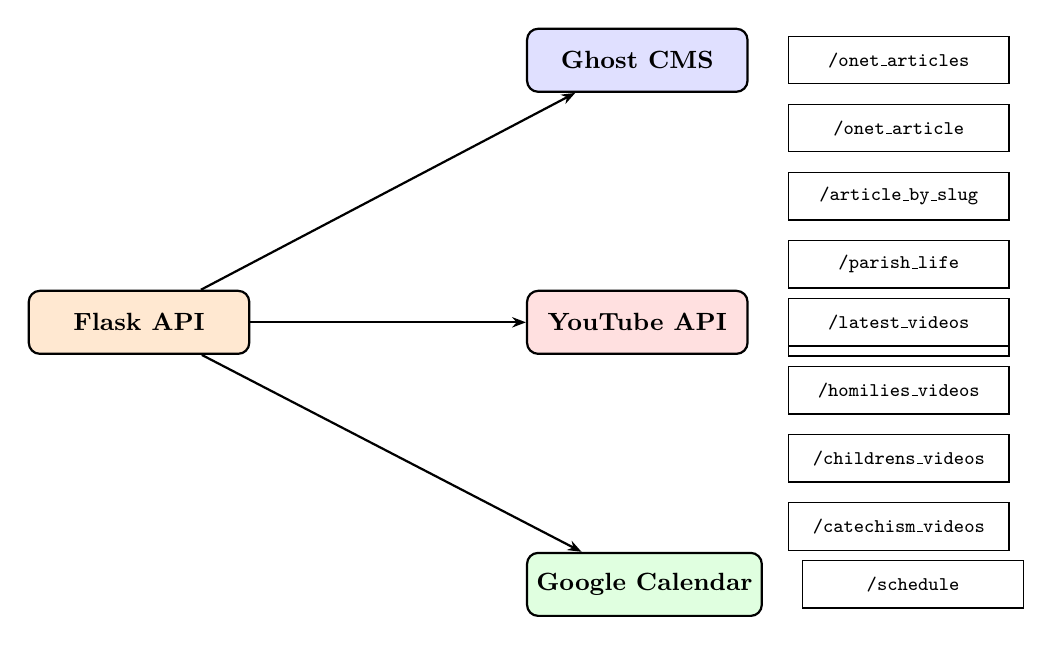
\begin{tikzpicture}[
    node distance=0.8cm and 2.2cm,
    group/.style={rectangle, rounded corners, draw, thick, minimum width=2.8cm, minimum height=0.8cm, align=center, font=\small\bfseries},
    ep/.style={rectangle, draw, fill=white, minimum width=2.8cm, minimum height=0.6cm, align=center, font=\scriptsize\ttfamily},
    arr/.style={-{Stealth[length=5pt]}, thick},
]
    \node[group, fill=orange!18] (app) {Flask API};

    % Articles group
    \node[group, fill=blue!12, above right=2.5cm and 3.5cm of app] (articles) {Ghost CMS};
    \node[ep, right=0.5cm of articles] (a1) {/onet\_articles};
    \node[ep, below=0.25cm of a1] (a2) {/onet\_article};
    \node[ep, below=0.25cm of a2] (a3) {/article\_by\_slug};
    \node[ep, below=0.25cm of a3] (a4) {/parish\_life};
    \node[ep, below=0.25cm of a4] (a5) {/motd};

    % Videos group
    \node[group, fill=red!12, right=3.5cm of app] (videos) {YouTube API};
    \node[ep, right=0.5cm of videos] (v1) {/latest\_videos};
    \node[ep, below=0.25cm of v1] (v2) {/homilies\_videos};
    \node[ep, below=0.25cm of v2] (v3) {/childrens\_videos};
    \node[ep, below=0.25cm of v3] (v4) {/catechism\_videos};

    % Calendar group
    \node[group, fill=green!12, below right=2.5cm and 3.5cm of app] (cal) {Google Calendar};
    \node[ep, right=0.5cm of cal] (c1) {/schedule};

    \draw[arr] (app) -- (articles);
    \draw[arr] (app) -- (videos);
    \draw[arr] (app) -- (cal);
\end{tikzpicture}
\caption{API endpoint groups mapped to their external data sources.}
\label{fig:endpoints}
\end{figure}

\subsection{System Endpoints}

\begin{longtable}{lll}
\toprule
\textbf{Method} & \textbf{Path} & \textbf{Description} \\
\midrule
GET & \texttt{/} & HTML welcome page \\
GET & \texttt{/heartbeat} & Health check; returns \texttt{\{"status":"ok"\}} \\
GET & \texttt{/docs} & Interactive Swagger UI (Flasgger) \\
GET & \texttt{/apispec.json} & Raw OpenAPI spec JSON \\
\bottomrule
\end{longtable}

\subsection{Article Endpoints (Ghost CMS)}

All article endpoints call the Ghost CMS Content API at:\\
\url{https://orthodox-net.ghost.io/ghost/api/content/}

\subsubsection{\texttt{GET /onet\_articles}}
Returns the full Ghost CMS response for all posts tagged \texttt{orthodox\_net}, including the \texttt{posts} array with title, HTML content, tags, and authors. No pagination on the Flask side (Ghost's default page size applies).

\subsubsection{\texttt{GET /onet\_article\_data}}
Returns article metadata \textbf{without} full HTML content. Paginates through all Ghost pages (100 per page) to collect every post. Response is an array of:
\begin{lstlisting}[language={}, basicstyle=\ttfamily\footnotesize, frame=none, numbers=none]
{
  "id": "652a8f969a71080001718f5b",
  "title": "Article Title",
  "excerpt": "Custom excerpt text...",
  "posted_at": "2024-01-15T12:00:00.000Z",
  "tags": ["orthodox_net", "parish_life"],
  "authors": ["Author Name"],
  "url": "https://orthodox-net.ghost.io/article-slug/"
}
\end{lstlisting}
\textbf{Note:} The \texttt{excerpt} field maps to Ghost's \texttt{custom\_excerpt}, not the auto-generated excerpt. Articles without a custom excerpt will have \texttt{null} here.

\subsubsection{\texttt{GET /onet\_article?article\_id=\{id\}}}
Fetches a single article by Ghost CMS ID. Returns:
\begin{lstlisting}[language={}, basicstyle=\ttfamily\footnotesize, frame=none, numbers=none]
{
  "title": "Article Title",
  "content": "<strong>Reformatted HTML...</strong>",
  "featured_image": "https://images.unsplash.com/..."
}
\end{lstlisting}
\textbf{Heading reformatting:} All \texttt{<h1>} through \texttt{<h6>} tags are replaced with \texttt{<strong>} tags. This is done in \texttt{fetch\_ghost.py:reformat\_headings()} to give the frontend full control over heading styles.

\subsubsection{\texttt{GET /article\_by\_slug?slug=\{slug\}}}
SEO-friendly article lookup. Returns the same structure as \texttt{/onet\_article} plus additional fields: \texttt{slug}, \texttt{id}, \texttt{tags} (raw Ghost tag objects), \texttt{authors} (raw Ghost author objects), \texttt{published\_at}.

\subsubsection{\texttt{GET /onet\_articles\_to\_list}}
Filtered article list. Fetches all \texttt{orthodox\_net} posts, then filters client-side for articles whose \texttt{primary\_tag.name} starts with \texttt{onet\_}. Returns array of \texttt{\{id, primary\_tag\_slug, title, excerpt\}}.

\subsubsection{\texttt{GET /parish\_life}}
Fetches all article metadata via \texttt{fetch\_tagged\_post\_data("orthodox\_net")}, filters for articles having both \texttt{orthodox\_net} and \texttt{parish\_life} tags, sorts by \texttt{posted\_at}, then fetches the full article content for the most recent one. Response matches \texttt{/onet\_article}.

\subsubsection{\texttt{GET /motd}}
Same logic as \texttt{/parish\_life} but filters for the \texttt{motd} tag instead.

\subsubsection{\texttt{GET /latest\_article?article\_id=\{id\}}}
Fetches the article list (calls \texttt{get\_article\_list()} internally, result unused) then fetches the article by ID. Functionally equivalent to \texttt{/onet\_article}.

\subsubsection{\texttt{GET /legacy\_article?filename=\{filename\}}}
Scrapes a legacy article from \url{https://www.orthodox.net/articles/{filename}.html}. Extracts content between \texttt{<!--BEGIN-CONTENT-->} and \texttt{<!--END-CONTENT-->} comment markers. Returns \texttt{\{"body":"..."\}} or an error if markers are not found.

\subsubsection{\texttt{GET /test\_article}}
Debug endpoint. Fetches article with hardcoded ID \texttt{652a8f969a71080001718f5b}. Not intended for production use.

\subsection{Video Endpoints (YouTube)}

YouTube integration uses channel ID \texttt{UCb\_MxJmD\_J4peQtRHj-qBKA} and the YouTube Data API v3. API key is loaded from \texttt{youtube\_credentials.py}.

\textbf{Common video response format} (all video endpoints return an array of these):
\begin{lstlisting}[language={}, basicstyle=\ttfamily\footnotesize, frame=none, numbers=none]
{
  "title": "Video Title",
  "description": "Video description...",
  "url": "https://www.youtube.com/watch?v=VIDEO_ID",
  "thumbnail": "https://i.ytimg.com/vi/.../hqdefault.jpg",
  "published_at": "2025-01-15T12:00:00Z",
  "channel_title": "Orthodox Net",
  "duration": "PT15M30S",
  "view_count": "1234",
  "like_count": "56",
  "dislike_count": "N/A"
}
\end{lstlisting}

\subsubsection{\texttt{GET /latest\_videos}}
\textbf{Cached.} Checks Supabase for videos with \texttt{video\_type='latest'} cached within 6 hours. On miss, calls YouTube Search API to get video IDs, then YouTube Videos API for full metadata, caches the raw response, and returns formatted data.

\textbf{YouTube API calls on cache miss:} 2 (one Search, one Videos).

\subsubsection{\texttt{GET /homilies\_videos}}
\textbf{Not cached.} Calls YouTube Playlist Items API for the Homilies playlist, then Videos API for metadata. Default 20 results.

\subsubsection{\texttt{GET /childrens\_videos}}
\textbf{Not cached.} Playlist \texttt{PLEh2brXYUf7nIigGqPthPFw4ApKiIu9zW}. Same flow as homilies.

\subsubsection{\texttt{GET /catechism\_videos}}
\textbf{Not cached.} Playlist \texttt{PLEh2brXYUf7k06I4K0dgAJC11A3TlgpFK}. Same flow as homilies.

\subsubsection{\texttt{GET /view\_video\_cache?video\_type=\{type\}}}
Admin/debug endpoint. Returns all cached videos (ignoring TTL). Optional \texttt{video\_type} filter. Response:
\begin{lstlisting}[language={}, basicstyle=\ttfamily\footnotesize, frame=none, numbers=none]
{
  "count": 150,
  "videos": [
    {"video_id":"...","title":"...","video_type":"latest",
     "cached_at":"...","published_at":"...","thumbnail_url":"..."}
  ]
}
\end{lstlisting}

\subsubsection{\texttt{POST /cache\_videos?video\_type=\{type\}\&max\_results=\{n\}}}
Admin endpoint to force-refresh the cache. Parameters:
\begin{itemize}
    \item \texttt{video\_type}: \texttt{latest}, \texttt{homilies}, \texttt{childrens}, \texttt{catechism}, or \texttt{all} (default: \texttt{latest})
    \item \texttt{max\_results}: 1--50 (default: 20, capped at 50)
\end{itemize}
For each type: clears existing cache entries, fetches fresh from YouTube, stores in Supabase. Returns count per type.

\subsection{Calendar Endpoint}

\subsubsection{\texttt{GET /schedule}}
Returns church events for the next 10 days. Uses US/Central timezone. Events are formatted as:
\begin{lstlisting}[language={}, basicstyle=\ttfamily\footnotesize, frame=none, numbers=none]
[
  {"date": "Sun - Dec 1", "time": "9am", "service": "Divine Liturgy"},
  {"date": "",             "time": "6pm", "service": "Vespers"}
]
\end{lstlisting}
The \texttt{date} field is an empty string for subsequent events on the same day (for display grouping). Times use 12-hour format with lowercase am/pm, minutes omitted when \texttt{:00}.

\textbf{Default Calendar ID:}\\
\texttt{s37s3qvlf9nobhplqp0umlcafs@group.calendar.google.com}\\
(overridable via \texttt{GOOGLE\_CALENDAR\_ID} env var).

%% ============================================================
\section{Core Module Details}
%% ============================================================

\subsection{Ghost CMS Integration (\texttt{fetch\_ghost.py})}

\textbf{Base URL:} \texttt{https://orthodox-net.ghost.io/ghost/api/content/}

\textbf{Authentication:} Content API key passed as \texttt{?key=} query parameter. Currently \textbf{hardcoded} in the source file (line 14).

\textbf{Key functions:}
\begin{itemize}
    \item \texttt{fetch\_posts()} --- All posts with tags and authors.
    \item \texttt{fetch\_tagged\_posts(slug)} --- Posts filtered by tag slug, single page.
    \item \texttt{fetch\_tagged\_post\_data(slug)} --- \textbf{Paginated} (100 per page). Returns metadata via \texttt{fetch\_ids\_from\_tagged\_post\_data()}.
    \item \texttt{fetch\_article(post\_id)} --- Single post; returns reformatted \texttt{\{title, content, featured\_image\}}.
    \item \texttt{fetch\_article\_by\_slug(slug)} --- Uses Ghost's \texttt{filter=slug:\{slug\}} query; returns extended fields.
    \item \texttt{reformat\_headings(content)} --- Replaces all heading tags (\texttt{h1}--\texttt{h6}) with \texttt{<strong>} so the frontend controls styling.
\end{itemize}

\textbf{Logging:} Writes to \texttt{fetch\_ghost.log} at DEBUG level.

\subsection{YouTube Integration (\texttt{fetch\_youtube.py})}

\textbf{API Key:} Loaded via \texttt{youtube\_credentials.get\_api\_key()}. Currently \textbf{hardcoded} in \texttt{youtube\_credentials.py}.

\textbf{API Endpoints Used:}
\begin{itemize}
    \item \texttt{youtube/v3/search} --- Channel search for latest videos (returns video IDs).
    \item \texttt{youtube/v3/playlistItems} --- Playlist items (returns video IDs).
    \item \texttt{youtube/v3/videos} --- Full video details (\texttt{snippet}, \texttt{statistics}, \texttt{contentDetails}).
\end{itemize}

\textbf{Key functions:}
\begin{itemize}
    \item \texttt{fetch\_latest\_videos()} --- Cache-aware. Checks the video cache for \texttt{'latest'} type, returns cached on hit. On miss: Search API $\rightarrow$ Videos API $\rightarrow$ cache $\rightarrow$ return.
    \item \texttt{fetch\_latest\_video\_ids(max\_results)} --- Search API call only.
    \item \texttt{fetch\_video\_data(video\_ids)} --- Videos API call; accepts comma-joined IDs.
    \item \texttt{fetch\_playlist\_video\_ids(playlist\_id, max\_results)} --- Playlist Items API.
    \item \texttt{fetch\_latest\_playlist\_videos(playlist\_id)} --- Playlist IDs $\rightarrow$ video details. Used by homilies/childrens/catechism endpoints.
    \item \texttt{fetch\_homilies\_playlist()}, \texttt{fetch\_childrens\_playlist()},\\ \texttt{fetch\_catechism\_playlist()} --- Convenience wrappers with hardcoded playlist IDs.
\end{itemize}

\subsection{Calendar Integration (\texttt{fetch\_calendar.py})}

Uses \texttt{google-api-python-client} with an API key (no OAuth). All times are processed in \textbf{US/Central} timezone.

\textbf{Key functions:}
\begin{itemize}
    \item \texttt{fetch\_calendar\_events()} --- Cache-aware main function. Calculates today~+~10 days in US/Central, checks cache, falls back to API. Handles pagination. Returns raw JSON string.
    \item \texttt{extract\_events(events\_json)} --- Formats raw Google Calendar events into display format (\texttt{date}/\texttt{time}/\texttt{service}). Handles all-day events, timezone conversion, date grouping (empty \texttt{date} for same-day events).
    \item \texttt{return\_calendar\_events()} --- Orchestrator; calls fetch then extract.
\end{itemize}

\subsection{Legacy Article Scraper (\texttt{fetch\_legacy\_article.py})}

Fetches HTML from \texttt{https://www.orthodox.net/articles/\{filename\}.html} with a browser-like User-Agent header. Extracts content between \texttt{<!--BEGIN-CONTENT-->} and \texttt{<!--END-CONTENT-->} comment markers. No caching. Logs to \texttt{fetch\_orthodox\_net.log}.

%% ============================================================
\section{Error Handling Patterns}
%% ============================================================

\subsection{General Pattern}
All \texttt{app.py} endpoints wrap their logic in try-except blocks and return structured JSON error responses:
\begin{itemize}
    \item \textbf{400} --- Missing required query parameters.
    \item \textbf{404} --- No data found (empty article list, no videos, no schedule).
    \item \textbf{500} --- Unhandled exceptions (logged, generic message returned).
\end{itemize}

\subsection{Cache Failure Resilience}
\begin{itemize}
    \item If Supabase credentials are missing, caching is silently disabled at module load. The app functions normally, just without caching.
    \item If a cache write fails (e.g., Supabase is down), a warning is logged but the response still returns fresh data.
    \item If the Google Calendar API fails, \texttt{fetch\_calendar.py} returns expired cached data if available, otherwise an empty array.
    \item If the YouTube API fails (missing \texttt{items} in response), an error message is printed and an empty list is returned.
\end{itemize}

\subsection{External API Errors}
\begin{itemize}
    \item Ghost CMS errors propagate as exceptions (no explicit status code checking in \texttt{fetch\_ghost.py}).
    \item YouTube errors are detected by checking for \texttt{"items"} key in response; error messages are extracted from \texttt{response.error.message}.
    \item Google Calendar uses the \texttt{googleapiclient} exception handling.
\end{itemize}

%% ============================================================
\section{Logging}
%% ============================================================

\begin{longtable}{lll}
\toprule
\textbf{Log File} & \textbf{Source Module} & \textbf{Level} \\
\midrule
\texttt{app.log} & \texttt{app.py} & DEBUG \\
\texttt{fetch\_ghost.log} & \texttt{fetch\_ghost.py} & DEBUG \\
\texttt{fetch\_orthodox\_net.log} & \texttt{fetch\_legacy\_article.py} & DEBUG \\
(console only) & \texttt{fetch\_calendar.py} & INFO \\
(console only) & \texttt{calendar\_cache.py} & INFO \\
(console only) & \texttt{video\_cache.py} & INFO \\
(console only) & \texttt{fetch\_youtube.py} & (module logger) \\
\bottomrule
\end{longtable}

All log files use the format: \texttt{\%(asctime)s - \%(levelname)s - \%(message)s}.

\texttt{app.py} configures dual output: file (\texttt{app.log}) + console via a \texttt{StreamHandler}.

\textbf{Cache-specific log messages to watch for:}
\begin{itemize}
    \item \texttt{"USING CACHED EVENTS"} / \texttt{"USING CACHED VIDEOS"} --- Cache hit.
    \item \texttt{"FETCHING FRESH"} --- Cache miss, calling external API.
    \item \texttt{"Successfully cached N events/videos"} --- Cache write succeeded.
    \item \texttt{"Failed to cache ... but continuing"} --- Cache write failed, non-fatal.
    \item \texttt{"Supabase credentials not found"} --- Caching disabled entirely.
\end{itemize}

%% ============================================================
\section{Environment Configuration}
%% ============================================================

The application loads environment variables from a \texttt{.env} file via \texttt{python-dotenv}. See \texttt{.env.sample} for the complete template.

\begin{longtable}{llp{7cm}}
\toprule
\textbf{Variable} & \textbf{Required} & \textbf{Description} \\
\midrule
\endhead
\texttt{GHOST\_BASE\_URL} & Yes* & Ghost CMS base URL. *Currently hardcoded; \texttt{.env.sample} is prepared for migration. \\
\texttt{GHOST\_API\_KEY} & Yes* & Ghost Content API key. *Currently hardcoded in \texttt{fetch\_ghost.py}. \\
\texttt{YOUTUBE\_API\_KEY} & Yes* & YouTube Data API v3 key. *Currently hardcoded in \texttt{youtube\_credentials.py}. \\
\texttt{YOUTUBE\_CHANNEL\_ID} & Yes* & YouTube channel ID. *Currently hardcoded in \texttt{fetch\_youtube.py}. \\
\texttt{YOUTUBE\_HOMILIES\_PLAYLIST} & No* & Homilies playlist ID. *Hardcoded. \\
\texttt{YOUTUBE\_CHILDRENS\_PLAYLIST} & No* & Children's playlist ID. *Hardcoded. \\
\texttt{YOUTUBE\_CATECHISM\_PLAYLIST} & No* & Catechism playlist ID. *Hardcoded. \\
\texttt{GOOGLE\_API\_KEY} & \textbf{Yes} & Google API key for Calendar. \textbf{Read from env at runtime.} \\
\texttt{GOOGLE\_CALENDAR\_ID} & No & Calendar ID. Default: \texttt{s37s3qvlf9nobhplqp0umlcafs@...} \\
\texttt{SUPABASE\_URL} & \textbf{Yes} & Supabase project URL. \textbf{Read from env at runtime.} \\
\texttt{SUPABASE\_KEY} & \textbf{Yes} & Supabase service role key. \textbf{Read from env at runtime.} \\
\texttt{SUPABASE\_DB\_URL} & No & Direct PostgreSQL connection string (used by \texttt{db/} setup scripts). \\
\texttt{RENDER} & Auto & Set automatically by Render.com. Detected by \texttt{app.py} to switch Swagger to HTTPS scheme. \\
\bottomrule
\end{longtable}

\textbf{Critical note:} Only \texttt{GOOGLE\_API\_KEY}, \texttt{SUPABASE\_URL}, and \texttt{SUPABASE\_KEY} are actually read from environment variables at runtime. Ghost CMS and YouTube credentials are \textbf{hardcoded in source files}. The \texttt{.env.sample} was created to support migrating these to env vars, but that migration has not been completed.

%% ============================================================
\section{Deployment \& DevOps}
%% ============================================================

\subsection{Hosting Platform}

The application is deployed on \textbf{Render.com}. The Render project is named \textbf{``orthodox.net Flask Backend''} and contains two environments, each with a single Web Service.

\textbf{Note:} The \texttt{Procfile} in the repository originated from an earlier Heroku deployment. Render also reads this format, so it remains functional. If Render-specific features are needed in the future (e.g., health check paths, pre-deploy commands), consider adding a \texttt{render.yaml} Blueprint.

\subsection{Render Environments}

\begin{figure}[p]
\centering
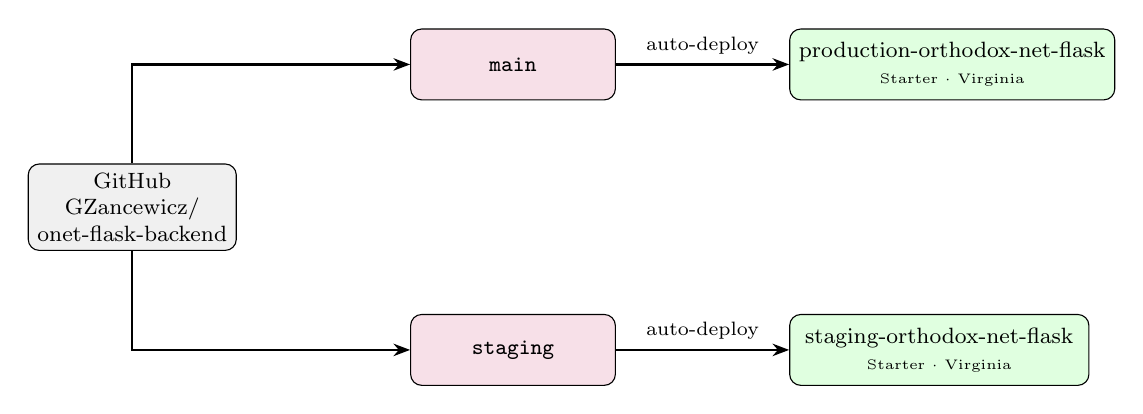
\begin{tikzpicture}[
    node distance=1.5cm and 1.8cm,
    box/.style={rectangle, draw, rounded corners, minimum width=2.6cm, minimum height=0.9cm, align=center, font=\footnotesize},
    repo/.style={box, fill=gray!12},
    branch/.style={box, fill=purple!12},
    env/.style={box, fill=green!12, minimum width=3.8cm},
    arr/.style={-{Stealth[length=6pt]}, thick},
]
    % GitHub
    \node[repo] (github) {GitHub\\GZancewicz/\\onet-flask-backend};

    % Branches
    \node[branch, above right=0.8cm and 2.2cm of github] (main) {\texttt{main}};
    \node[branch, below right=0.8cm and 2.2cm of github] (staging) {\texttt{staging}};

    % Render services
    \node[env, right=2.2cm of main] (prod) {production-orthodox-net-flask\\{\tiny Starter $\cdot$ Virginia}};
    \node[env, right=2.2cm of staging] (stag) {staging-orthodox-net-flask\\{\tiny Starter $\cdot$ Virginia}};

    % Arrows
    \draw[arr] (github) |- (main);
    \draw[arr] (github) |- (staging);
    \draw[arr] (main) -- node[above, font=\scriptsize] {auto-deploy} (prod);
    \draw[arr] (staging) -- node[above, font=\scriptsize] {auto-deploy} (stag);
\end{tikzpicture}
\caption{Deployment pipeline. Render watches each branch on GitHub and auto-deploys on push. Production: \texttt{https://production-orthodox-net-flask.onrender.com}. Staging: \texttt{https://staging-orthodox-net-flask.onrender.com}.}
\label{fig:deployment}
\end{figure}

\subsubsection{Production Environment}

\begin{longtable}{lp{9cm}}
\toprule
\textbf{Property} & \textbf{Value} \\
\midrule
Render service name & \texttt{production-orthodox-net-flask} \\
Service type & Web Service \\
Service ID & \texttt{srv-d2ce9g0gjchc7382590g} \\
Plan & Starter \\
Runtime & Python 3 \\
Region & Virginia (US East) \\
Git branch & \texttt{main} \\
Live URL & \url{https://production-orthodox-net-flask.onrender.com} \\
Swagger docs & \url{https://production-orthodox-net-flask.onrender.com/docs} \\
Auto-deploy & On push to \texttt{main} \\
Manual deploy & Available via Render dashboard (``Manual Deploy'' button) \\
\bottomrule
\end{longtable}

\subsubsection{Staging Environment}

\begin{longtable}{lp{9cm}}
\toprule
\textbf{Property} & \textbf{Value} \\
\midrule
Render service name & \texttt{staging-orthodox-net-flask} \\
Service type & Web Service \\
Service ID & \texttt{srv-d2caeg9r0fns73dpbne0} \\
Plan & Starter \\
Runtime & Python 3 \\
Region & Virginia (US East) \\
Git branch & \texttt{staging} \\
Live URL & \url{https://staging-orthodox-net-flask.onrender.com} \\
Swagger docs & \url{https://staging-orthodox-net-flask.onrender.com/docs} \\
Auto-deploy & On push to \texttt{staging} \\
\bottomrule
\end{longtable}

\subsection{Render Service Configuration}

Both services share the same build and runtime configuration:

\begin{longtable}{ll}
\toprule
\textbf{Setting} & \textbf{Value} \\
\midrule
Build command & \texttt{pip install -r requirements.txt} \\
Start command & \texttt{gunicorn app:app} (from \texttt{Procfile}) \\
Python version & 3.12.3 (from \texttt{runtime.txt}) \\
Environment variables & Configured per-service in Render dashboard \\
HTTPS & Provided automatically by Render \\
CORS & Open to all origins (\texttt{origins: "*"}) \\
\bottomrule
\end{longtable}

\textbf{Environment variables} are configured separately for each service in the Render dashboard and are \textbf{not stored in the repository}. Both services need the same set of variables (\texttt{GOOGLE\_API\_KEY}, \texttt{SUPABASE\_URL}, \texttt{SUPABASE\_KEY}, etc.), but staging may point to different Supabase projects or use different API keys for isolation.

Render automatically sets the \texttt{RENDER} environment variable, which the application detects to switch Swagger UI to HTTPS mode.

\subsection{Deployment Workflow}

\begin{enumerate}
    \item \textbf{Feature development:} Create a feature branch from \texttt{main}, make changes, open a PR against \texttt{main}.
    \item \textbf{Staging test:} Merge the PR into \texttt{staging} (or push the feature branch to \texttt{staging}) to trigger a staging deploy. Verify at \url{https://staging-orthodox-net-flask.onrender.com}.
    \item \textbf{Production release:} Merge the PR into \texttt{main}. Render auto-deploys to production.
    \item \textbf{Rollback:} Use Render's ``Manual Deploy'' to redeploy a previous commit, or revert the Git commit and push.
\end{enumerate}

\subsection{Procfile}

The \texttt{Procfile} contains: \texttt{web: gunicorn app:app}

This format originated with Heroku but Render also supports it. No Gunicorn worker count or timeout is specified, so Render/Gunicorn defaults apply. For higher traffic, consider adding \texttt{-w 4 --timeout 120}.

\subsection{CORS Configuration}

CORS is configured in \texttt{app.py} as:
\begin{lstlisting}[basicstyle=\ttfamily\footnotesize]
CORS(app, resources={r"/*": {"origins": "*"}})
\end{lstlisting}
This allows \textbf{any origin} to make requests. This is intentional --- the API is designed to be consumed by frontend applications running on different domains.

\subsection{Swagger / HTTPS Detection}

\texttt{app.py} detects the Render environment and adjusts the Swagger spec:
\begin{lstlisting}[basicstyle=\ttfamily\footnotesize]
is_production = os.environ.get('RENDER') is not None
swagger_template = {
    ...
    "schemes": ["https"] if is_production else ["http", "https"],
}
\end{lstlisting}
This ensures the Swagger ``Try it out'' feature uses HTTPS in production.

%% ============================================================
\section{Development Setup}
%% ============================================================

\subsection{Quick Start}
\begin{enumerate}
    \item Clone the repository:\\
    \texttt{git clone https://github.com/GZancewicz/onet-flask-backend.git}
    \item \texttt{pip install -r requirements.txt}
    \item \texttt{cp .env.sample .env} and fill in credentials\\(at minimum: \texttt{GOOGLE\_API\_KEY}, \texttt{SUPABASE\_URL}, \texttt{SUPABASE\_KEY}).
    \item Run SQL from \texttt{db\_schema.sql} and \texttt{video\_cache\_schema.sql} in Supabase SQL editor.
    \item \texttt{python3 app.py} --- server starts at \texttt{http://localhost:5001}.
    \item Visit \texttt{http://localhost:5001/docs} for Swagger UI.
\end{enumerate}

\textbf{Note:} Ghost CMS and YouTube will work without \texttt{.env} changes because their credentials are currently hardcoded. Supabase and Google Calendar require valid env vars.

\subsection{Running Tests}
\begin{lstlisting}[language=bash, basicstyle=\ttfamily\footnotesize, frame=none, numbers=none]
pytest                          # Run all tests
pytest --cov                    # Run with coverage
pytest test/test_filename.py    # Run specific test file
\end{lstlisting}

\subsection{Test Organization}

\begin{longtable}{lp{8cm}}
\toprule
\textbf{Directory} & \textbf{Contents} \\
\midrule
\texttt{test/} & Main test suite: calendar fetch tests, database setup tests \\
\texttt{modules/youtube/test/} & YouTube module tests (unit tests with mocks + live API tests) \\
\texttt{legacy\_test/ghost/} & Ghost CMS tests: fetch article, posts, tags, tagged posts \\
\texttt{legacy\_test/youtube/} & Legacy YouTube tests: playlists, video data, latest videos \\
\texttt{db/test/} & Database setup and YouTube table creation tests \\
\bottomrule
\end{longtable}

Tests use \texttt{pytest-mock} to mock external API calls. Tests with ``live'' in the filename make actual API calls and may fail if API keys are invalid or quotas are exhausted.

\subsection{Compiling This Document}
\begin{lstlisting}[language=bash, basicstyle=\ttfamily\footnotesize, frame=none, numbers=none]
./compile_doc.sh    # Requires pdflatex (e.g., brew install basictex)
\end{lstlisting}

%% ============================================================
\section{Security Considerations}
\label{sec:security}
%% ============================================================

\begin{itemize}
    \item \textbf{Hardcoded API keys:} The Ghost CMS Content API key is hardcoded in \texttt{fetch\_ghost.py} (line~14). The YouTube API key is hardcoded in \texttt{youtube\_credentials.py} (line~1). Both are committed to Git. The Ghost key is read-only (low-risk by design), but the YouTube key should be migrated to an environment variable.
    \item \textbf{CORS wildcard:} All origins are allowed (\texttt{*}). This is by design but means the API is callable from any website.
    \item \textbf{No authentication:} The API has no authentication or rate limiting. All endpoints are public. The \texttt{POST /cache\_videos} admin endpoint is also unauthenticated.
    \item \textbf{No input sanitization on query params:} Parameters like \texttt{article\_id}, \texttt{slug}, and \texttt{filename} are passed directly to external APIs. The Ghost API and URL encoding provide some protection, but there is no explicit validation.
    \item \textbf{Supabase service role key:} The \texttt{SUPABASE\_KEY} used is the service role key (full access), not the anon key. This is appropriate for a backend but must never be exposed to the frontend.
    \item \textbf{Legacy article fetching:} The \texttt{filename} parameter in \texttt{/legacy\_article} is URL-encoded but not validated against a whitelist. It constructs a URL to \texttt{orthodox.net}.
\end{itemize}

%% ============================================================
\section{Known Technical Debt}
%% ============================================================

\begin{enumerate}
    \item \textbf{Hardcoded credentials} --- Ghost and YouTube credentials should be migrated to environment variables. The \texttt{.env.sample} is already prepared for this.
    \item \textbf{Inconsistent caching} --- Only \texttt{/latest\_videos} uses automatic caching. The playlist endpoints (\texttt{/homilies\_videos}, etc.) hit YouTube on every request and could benefit from the same pattern.
    \item \textbf{Duplicate YouTube table schemas} --- Both \texttt{db\_schema.sql} and \texttt{video\_cache\_schema.sql} define a \texttt{youtube\_videos} table with different columns. The simpler schema is what the code uses.
    \item \textbf{Backup/dead files} --- Several files appear unused: \texttt{app\_backup.py}, \texttt{app\_swagger\_hybrid.py}, \texttt{fetch\_youtube\_v0.py}, and others.
    \item \textbf{Dual Supabase clients} --- Both cache modules independently create Supabase clients at import time. A shared client would reduce overhead.
    \item \textbf{Separate logging configs} --- Each module calls \texttt{logging.basicConfig()} independently, which can conflict. A centralized setup would be better.
    \item \textbf{No rate limiting or auth} --- The \texttt{POST /cache\_videos} admin endpoint is publicly accessible with no authentication.
    \item \textbf{Ghost pagination inconsistency} --- \texttt{fetch\_tagged\_posts()} returns a single page, while \texttt{fetch\_tagged\_post\_data()} paginates through all pages. This means \texttt{/onet\_articles} may not return all articles.
    \item \textbf{Procfile} --- Originally for Heroku; still functional on Render but may cause confusion. Consider documenting or replacing with a \texttt{render.yaml} if Render-specific features are needed.
\end{enumerate}

%% ============================================================
\section{Maintenance Checklist}
\label{sec:checklist}
%% ============================================================

If taking over maintenance of this project, ensure you have the following:

\begin{enumerate}
    \item \textbf{GitHub access:} Write access to the repository at\\
    \url{https://github.com/GZancewicz/onet-flask-backend}

    \item \textbf{Render.com access:} Dashboard access to the ``orthodox.net Flask Backend'' project (both production and staging services --- logs, environment variables, manual deploys)

    \item \textbf{Render environment variables:} The values for \texttt{GOOGLE\_API\_KEY}, \texttt{SUPABASE\_URL}, and \texttt{SUPABASE\_KEY} configured in each Render service. These are not stored in the repository.

    \item \textbf{Supabase access:} Login to the Supabase project used for caching. Required for viewing cached data, running SQL, or modifying table schemas.

    \item \textbf{Ghost CMS access:} Admin login for the Ghost instance at \texttt{orthodox-net.ghost.io} for article and content management.

    \item \textbf{Google API credentials:} Access to the Google Cloud project that owns the API key used for Google Calendar. Required for quota monitoring and key rotation.

    \item \textbf{YouTube API credentials:} The YouTube Data API key (currently hardcoded in \texttt{youtube\_credentials.py}). Access to the Google Cloud project for quota monitoring.

    \item \textbf{DNS:} Understanding of who manages DNS for \texttt{orthodox.net}, in case the API needs a custom domain or subdomain in the future.

    \item \textbf{Hardcoded credentials:} Be aware that Ghost and YouTube API keys are hardcoded in source files, not read from environment variables. See Section~\ref{sec:security} for details.

    \item \textbf{Cache monitoring:} Familiarity with the Supabase tables (\texttt{calendar\_events}, \texttt{youtube\_videos}) and how to verify cache freshness. The admin endpoints \texttt{GET /view\_video\_cache} and \texttt{POST /cache\_videos} can be used without Supabase dashboard access.
\end{enumerate}

%% ============================================================
\clearpage
\appendix
\section{Project History by Milestone}
\label{sec:history}
%% ============================================================

This appendix summarizes the development history of the orthodox.net Flask Backend organized by major milestone. The full commit history is available via \texttt{git log} on the \texttt{main} branch at \url{https://github.com/GZancewicz/onet-flask-backend}.

\subsection{Phase 1: Initial Setup and Core API (Sep 2023)}

The project began on September 3, 2023, bootstrapping the Flask backend with initial endpoints and deploying to Heroku.

\begin{itemize}
    \item Created the Flask application with CORS support and a \texttt{/heartbeat} health check
    \item Copied utility scripts from the earlier \texttt{onet-v2} project
    \item Built the \texttt{/schedule} endpoint, initially parsing legacy bulletin data, then switching to the Google Calendar API
    \item Integrated YouTube video fetching via the YouTube Data API v3
    \item Configured Heroku deployment with \texttt{Procfile} and \texttt{requirements.txt}
    \item Resolved CORS issues for cross-origin frontend access
\end{itemize}

\subsection{Phase 2: YouTube Playlists and Ghost CMS (Oct--Nov 2023)}

Extended the API with curated video playlists and began integrating Ghost CMS for article management.

\begin{itemize}
    \item Added YouTube playlist support for homilies, children's sermons, and catechism videos
    \item Built the Ghost CMS Content API interface (\texttt{fetch\_ghost.py})
    \item Created \texttt{/test\_article} and \texttt{/onet\_articles} endpoints
    \item Added \texttt{/onet\_article?article\_id=} for fetching individual articles
    \item Implemented heading reformatting to give the frontend control over styles
\end{itemize}

\subsection{Phase 3: Article Features and Metadata (Jan--Jul 2024)}

Expanded article functionality with metadata endpoints and new content types.

\begin{itemize}
    \item Added \texttt{/latest\_article} endpoint
    \item Updated API keys and added new article endpoints
    \item Built article metadata extraction (title, excerpt, tags, authors)
    \item Developed the \texttt{/onet\_article\_data} endpoint for lightweight article listings
\end{itemize}

\subsection{Phase 4: Testing, Database, and Infrastructure (Dec 2024)}

Major infrastructure push: introduced testing, database integration, and dependency management.

\begin{itemize}
    \item Added unit testing with \texttt{pytest} and \texttt{pytest-mock} (PR~\#1)
    \item Set up Ghost CMS unit tests
    \item Configured PostgreSQL database and YouTube SQL tables via SQLAlchemy
    \item Set up \texttt{python-dotenv} for credential management
    \item Pinned \texttt{Werkzeug} version to resolve Heroku deployment errors
    \item Built YouTube video table population (100 latest videos)
    \item Added test coverage reporting with \texttt{pytest-cov}
    \item Created playlist video retrieval from the database
    \item Added home page, \texttt{/onet\_article\_data} URL field, and feature image support
    \item Built legacy article scraping from \texttt{orthodox.net} (PR~\#5)
\end{itemize}

\subsection{Phase 5: Content Endpoints and Calendar (Jan--Feb 2025)}

Added parish-specific content features and improved the calendar.

\begin{itemize}
    \item Extended calendar to fetch events 10 days out (PR~\#6)
    \item Stopped tracking log files in Git
    \item Added \texttt{/parish\_life} endpoint for parish life articles (PR~\#7)
    \item Added \texttt{/motd} endpoint for message of the day (PR~\#8)
    \item Removed article count limits on \texttt{/onet\_article\_data} (PR~\#9)
\end{itemize}

\subsection{Phase 6: Migration to Render and Supabase Caching (Aug 2025)}

Major platform migration from Heroku to Render, with Supabase caching layer.

\begin{itemize}
    \item Migrated hosting from Heroku to Render.com with staging and production environments
    \item Added Swagger UI documentation via Flasgger at \texttt{/docs}
    \item Recovered \texttt{/article\_by\_slug} endpoint for SEO-friendly URLs
    \item Moved Google Calendar credentials to environment variables
    \item Integrated Supabase as the caching layer for calendar events (24-hour TTL)
    \item Added video caching in Supabase for \texttt{/latest\_videos} (6-hour TTL)
    \item Fixed Swagger HTTPS scheme detection for Render
    \item Built \texttt{POST /cache\_videos} admin endpoint and \texttt{/view\_video\_cache}
    \item Created \texttt{video\_cache.py} and \texttt{calendar\_cache.py} modules (PR~\#10, \#12)
\end{itemize}

\subsection{Phase 7: Stabilization and Bug Fixes (Dec 2025)}

Polished caching, fixed pagination bugs, and improved project hygiene.

\begin{itemize}
    \item Enhanced caching features and updated README
    \item Updated \texttt{.gitignore} to ignore all \texttt{.env} files
    \item Fixed bug where \texttt{fetch\_tagged\_post\_data()} was limited to one page of Ghost results, causing missing blog posts (PR~\#14)
\end{itemize}

%% ============================================================
\clearpage
\section{Document Revision History}
\label{sec:revisions}
%% ============================================================

\begin{longtable}{llp{9.5cm}}
\toprule
\textbf{Version} & \textbf{Date} & \textbf{Description} \\
\midrule
\endhead
1.0 & 2025-05-04 & Initial document creation. Basic overview of system architecture, API endpoints, core modules, logging, and deployment. Created as both \texttt{onet\_backend.tex} and \texttt{technical\_documentation.tex} (identical duplicates). \\
\addlinespace
2.0 & 2026-03-15 & Comprehensive rewrite. Removed duplicate \texttt{technical\_documentation.tex}. Added executive summary, complete API reference with request/response examples, full database schemas (SQL), caching layer details with TTL and fallback behavior, module dependency graph, Supabase client initialization patterns, error handling patterns, environment variable reference table, security considerations, known technical debt (9 items). Added Render.com deployment details with service IDs, URLs, and deployment workflow. Added TikZ diagrams (system architecture, module dependencies, cache flow, endpoint map, deployment pipeline). Added project history appendix (7 phases). Renamed ``Orthodox Net'' to ``orthodox.net'' throughout. Moved files to \texttt{doc/latex/onet\_backend/}. \\
\bottomrule
\end{longtable}

\end{document}
